

\title{Crowdflow Dataset -- diluted pedestrian dynamics in the Metaforum building of Eindhoven University of Technology}
\author{
  Alessandro Corbetta \\
  \textit{Department of Applied Physics}\\
  \textit{Eindhoven University of Technology}\\
  \texttt{a.corbetta@tue.nl}\\  
  \and
  \\
  Federico Toschi\\
  \textit{Department of Applied Physics and}\\
  \textit{Department of Mathematics and Computer Science}\\
  \textit{Eindhoven University of Technology}\\
}

\documentclass[12pt]{article}

\usepackage{framed}
\usepackage{verbatim}
\usepackage{hyperref}
\usepackage{graphicx}
\graphicspath{ {../imgs/} }

\begin{document}
\date{2017}
\maketitle


\section{Dataset DOI and official download link}

\textbf{\url{https://doi.org/10.4121/uuid:25289586-4fda-4931-8904-d63efe4aa0b8}}\\


\noindent \textit{Reference publication:}\\
\verb|[1]| \href{http://journals.aps.org/pre/abstract/10.1103/PhysRevE.95.032316}{A. Corbetta, C. Lee, R. Benzi, A. Muntean, F. Toschi. \textbf{Fluctuations around mean walking behaviours in diluted pedestrian flows.} Phys. Rev. E. 95, 032316, 2017}\\

\noindent \textit{Usage and basic scripts:}\\
\url{https://github.com/crowdflowTUe/MF_landing_data_analysis}




\begin{figure}[h]

  \centering
  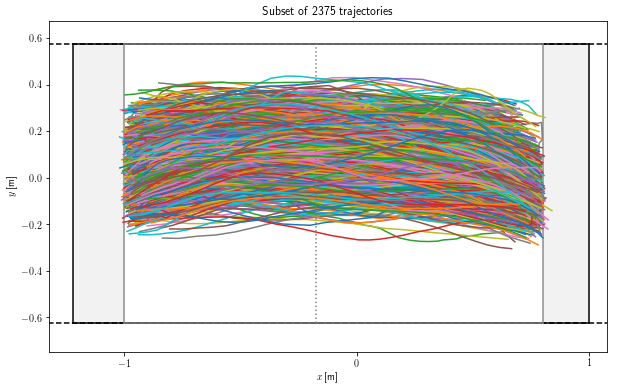
\includegraphics[width=0.75\textwidth, trim={0cm 0 0 .7cm },clip]{traj_portrait.png}
    \caption{Random subset of about $2300$ trajectories in the dataset.\label{fig}}
\end{figure}




\section{Dataset description}

This is a dataset of pedestrian trajectories recorded on a nearly 24/7 schedule in a landing in the Metaforum building at Eindhoven University of Technology. The data acquisition spanned over a year and, overall, about $250.000$ trajectories have been collected. Depth imaging data has been first obtained via an overhead Microsoft Kinect sensor, then ad hoc localization algorithms and Particle Tracking Velocimetry-like tracking have been employed to estimate the trajectory of individual heads (cf. [1]). The current dataset includes $20.000$ trajectories from pedestrians walking undisturbed i.e. in diluted conditions (individuals are walking alone in the facility, see Fig.~\ref{fig}). There are $10.000$ trajectories of pedestrians crossing the landing entering from the left hand side (file: ``left-to-right.ssv'') and $10.000$ trajectories of pedestrians entering in the opposite side (file: ``right-to-left.ssv'', right-left reference is given according to [1]). The purpose of the dataset is to enable ensemble analyses of diluted pedestrian motion.

\noindent The trajectories are in the following table format: \\

\verb|Pid  Rstep  X  Y  X_SG  Y_SG  U_SG  V_SG| \\

\noindent where:
\begin{itemize}
  \item \verb|Pid|: unique identifier of a trajectory
  \item \verb|Rstep|: identifier of the timestep (starts from zero, the first $5$ and last $5$ samples are eliminated as typically less precise)
  \item \verb|X,Y|: position in Cartesian coordinates (in meters)
  \item \verb|X_SG,Y_SG|: position in Cartesian coordinates after Savizky-Golay smoothing (in meters, cf. paper) 
  \item \verb|U_SG, V_SG|: velocity in Cartesian coordinates after Savizky-Golay smoothing (in meters per second, cf. paper).
\end{itemize}

\noindent To use the dataset please cite \href{http://journals.aps.org/pre/abstract/10.1103/PhysRevE.95.032316}{[1]} as well as this dataset (DOI: \url{https://doi.org/10.4121/uuid:25289586-4fda-4931-8904-d63efe4aa0b8}).


\end{document}
